\section{Morfeas WEB NOx-if/Portal UI}
The Morfeas WEB NOx-if/Portal can be accessed from the "Morfeas WEB" front page by clicking in the dedicated button (NOXs Portal).
A new window will open with the Morfeas WEB NOx-if Portal.
Then select from top-left corner the CAN-if name and the UniNOx address on interest.
At figure \ref{fig:NOX-if_UI} shown a example view.

\begin{figure}[h]
\centering
	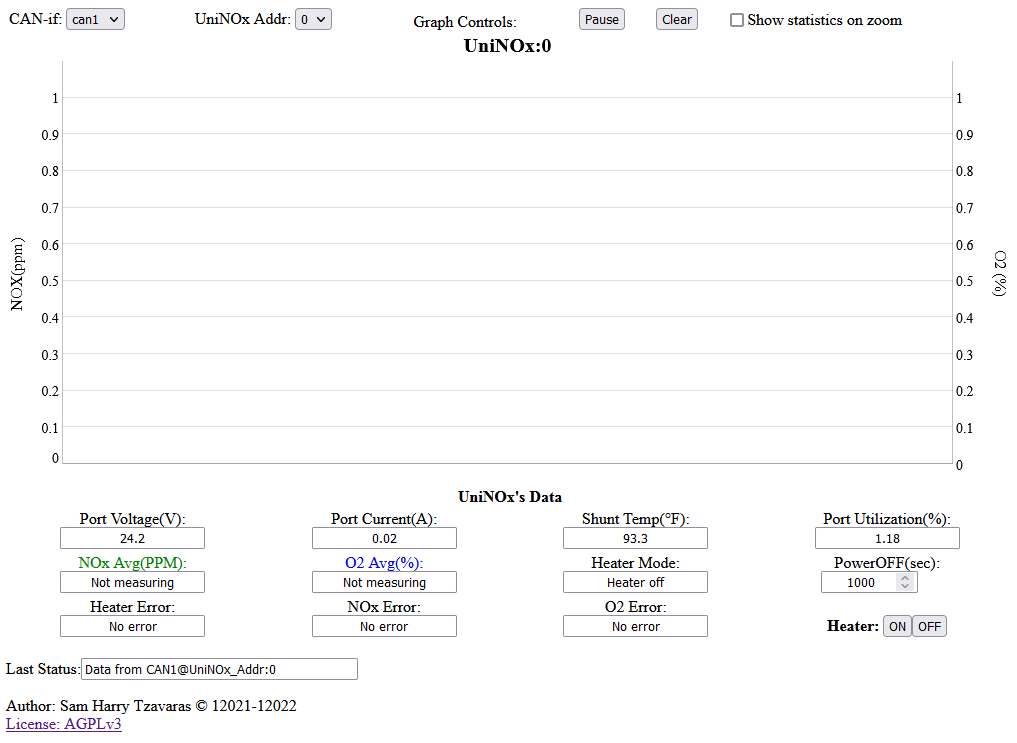
\includegraphics[width=3.5in,angle=0]{../art/Morfeas_web_if/Morfeas_web_NOX_if_UI.png}
	\caption{Morfeas WEB NOX-if UI}
	\label{fig:NOX-if_UI}
\end{figure}

The Morfeas WEB NOx-if Portal split in two sections. The Upper section contains the graph and some controls related to it.
At the lower section, provided live information related to the CAN-if power supply section and the UNiNOx on interest.

To start a measurement the heater of the UNiNOx sensor must be energized. This done from the button at the right bottom corner.
To energize/de-energize both UNiNOx (in case that are two in chain) you can press and hold the \textbf{"Shift"} key.
In addition to this an autoPowerOFF mechanism is provided, the value of the \textbf{"PowerOFF(sec)"} field is set the autoPowerOFF time in seconds.
\begin{figure}[h]
\centering
	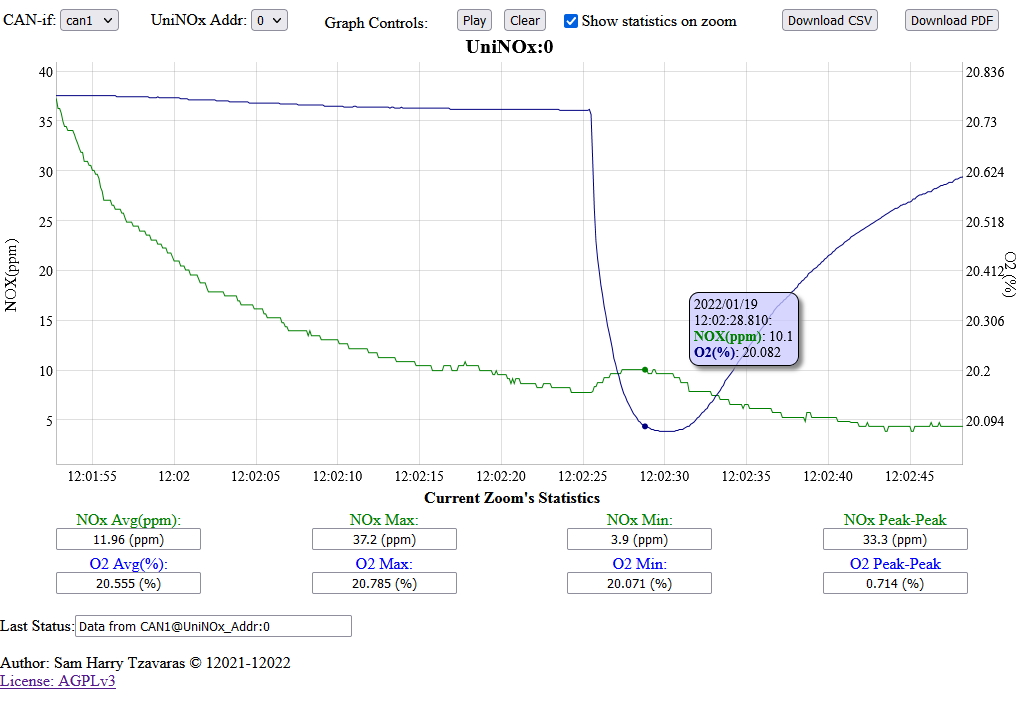
\includegraphics[width=3.5in,angle=0]{../art/Morfeas_web_if/Morfeas_web_NOX_if_UI_zoom.png}
	\caption{Morfeas WEB NOX-if UI Zoom mode}
	\label{fig:NOX-if_UI_zoom}
\end{figure}
The graph show the valid reading from the sensor. A zoom in mechanism is provided with purpose to provide further examination of the graph.
This mechanism works by click and select a portion of the graph (ex. figure \ref{fig:NOX-if_UI_zoom}).

In the zoom mode two button shall appeared at the top-right corner with functions export of the zoom data in ".csv" and ".pdf" formats.
The "Show statistics on zoom" option have function to replace the lower section with statistics for the zoomed area.
To exit zoom mode do double click on graph.